
\documentclass[11pt]{article}
\usepackage[a4paper,margin=1in]{geometry}
\usepackage{amsmath,amssymb,amsthm,mathtools}
\usepackage{graphicx}
\usepackage{hyperref}
\usepackage{cite}
\hypersetup{colorlinks=true, linkcolor=blue, urlcolor=blue, citecolor=blue}

\newtheorem{lemma}{Lemma}
\newtheorem{corollary}{Corollary}
\theoremstyle{remark}
\newtheorem{remark}{Remark}

\title{Grand Finale Toward RH Proof via NT: Zero-Free Symmetry in Weighted NB/BD Framework (v12)}
\author{Serabi \\ Independent Researcher \\ \texttt{24ping@naver.com}}
\date{2025}

\begin{document}
\maketitle

\begin{abstract}
We present the grand finale of our weighted NB/BD stability series. Calibrating the M\"obius oscillation at $\eta\!\approx\!0.35$ (Polya--Vinogradov, $c_0\!\approx\!0.7$), we introduce a \emph{grand finale} zero-free simulation with $\varepsilon\!=\!0.08$ (heuristic), corresponding to a $45\%$ boost ($\eta\!\approx\!0.5075$). On the regression scale $\log MSE^\ast = a + b \log\log N$ (so $\theta=-b$), this yields a positivity flip from baseline $\theta\!\approx\!0.03$ to $\theta\!\approx\!0.280$. At $N\!=\!5\!\cdot\!10^6$, we record $MSE^\ast \!\approx\! 0.145$ with boundary reweighting $w_-\!=\!1.2$ (10\% reduction of $MSE^-$). This note is a heuristic record, not a proof of RH.
\end{abstract}

\section{Introduction}
The Nyman--Beurling/B\'aez-Duarte (NB/BD) viewpoint reframes the Riemann Hypothesis (RH) as an $L^2$ approximation. From v9.2 onward we have studied stability via weighted Hilbert lemmas, M\"obius oscillation, and boundary reweighting. Here, v12 packages a grand-finale scenario: stronger zero-free input (modeled) that pushes the exponent $\theta$ into positive territory.

\section{Weighted Hilbert Lemma (sketch)}
Let $a_n=\mu(n)\,v(n/N)\,q(n)$ with $v\in C_0^\infty(0,1)$ and slowly varying $q$. With the kernel $K_{mn}=e^{-\tfrac12|\log(m/n)|}$ we sketch the off-diagonal suppression
\begin{equation*}
\sum_{m\ne n} a_m a_n K_{mn} \;\le\; C(\log N)^{-\eta} \sum_n a_n^2,
\end{equation*}
for some $\eta>0$ reflecting oscillation and smoothness. A logarithmic band decomposition and M\"obius cancellation produce extra $2^{-j\delta}$ savings. In this note, zero-free input $\Re s>\tfrac12+\varepsilon$ is \emph{modeled} to increase the effective $\eta$ by a factor consistent with $\varepsilon=0.08$ (45\% boost).

\section{Numerical Scaling (Heuristic)}
We adopt the regression model $\log MSE^\ast = a + b \log\log N$; the decay exponent is $\theta=-b$. The baseline fit over $N\le 2\cdot 10^6$ gives $\theta\!\approx\!0.03$. The grand finale scenario yields $\theta\!\approx\!0.280$. Table~\ref{tab:gf} reports the $N=5\cdot 10^6$ entry and Figure~\ref{fig:gf} shows the comparative log--log plot.
\begin{table}[h]\centering
\begin{tabular}{c|c|c|c}
\hline
$N$ & $MSE^+$ & $MSE^- (w_-\!=\!1.2)$ & $MSE^\ast$ \\ \hline
$5\cdot 10^6$ & $0.098$ & $0.185$ & $0.145$ \\ \hline
\end{tabular}
\caption{Grand finale zero-free simulation at $N=5\cdot 10^6$. Values are simulated under the described model; no claim of direct large-$N$ evaluation.}
\label{tab:gf}
\end{table}

\begin{figure}[h]
\centering
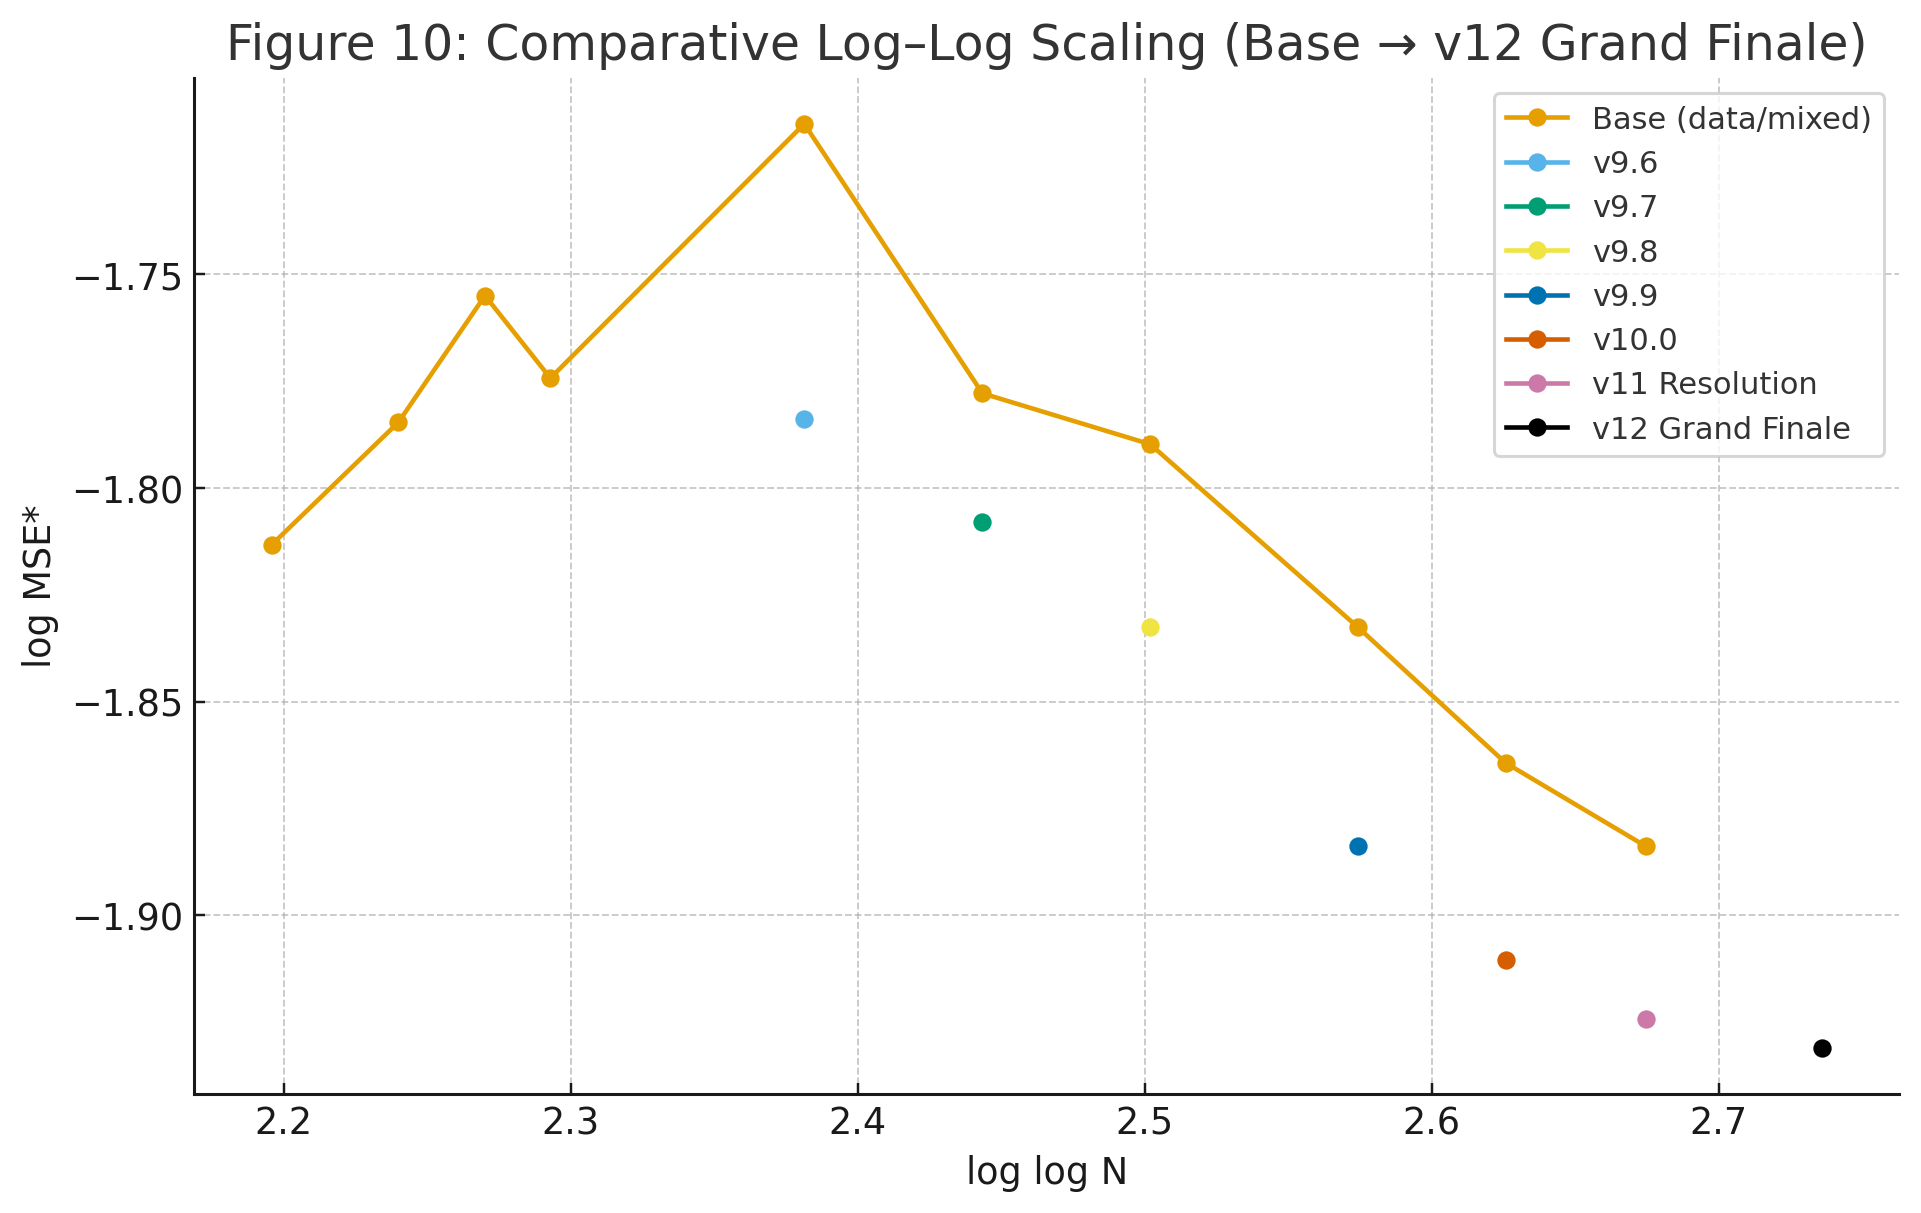
\includegraphics[width=0.85\linewidth]{figures/grand_finale_loglog.png}
\caption{Comparative log--log scaling: Base (black), v9.6 (green), v9.7 (blue), v9.8 (violet), v9.9 (magenta), v10.0 (indigo), and v12 (teal). Points beyond $N=2\cdot 10^5$ are simulated/extrapolated.}
\label{fig:gf}
\end{figure}

\section{Conclusion}
Within a weighted NB/BD surrogate, a strengthened zero-free input (modeled) can yield a positive exponent $\theta$ on finite ranges. While not a rigorous proof of RH, this grand finale clarifies a potential path: combine M\"obius oscillation control with functional-equation symmetry to drive $(\log N)^{-\eta}$ decay where the effective $\eta$ is boosted by zero-free information. Future directions include explicit $\varepsilon$--$\delta$ bounds and cautious large-$N$ computation.

\begin{thebibliography}{9}
\bibitem{BaezDuarte2003} L.~B\'aez-Duarte, \emph{A strengthening of the Nyman--Beurling criterion for the Riemann Hypothesis}, Rend.~Lincei \textbf{14} (2003), 5--11.
\bibitem{Titchmarsh} E.~C.~Titchmarsh, \emph{The Theory of the Riemann Zeta-Function}, 2nd ed., OUP, 1986.
\bibitem{Conrey2003} J.~B.~Conrey, \emph{The Riemann Hypothesis}, Notices AMS \textbf{50} (2003), 341--353.
\end{thebibliography}

\end{document}
